\chapter{Basic Data  Structures}


\section{Introduction}
Abstract Data Types (ADT):
\begin{enumerate}
\item Queue
\item Stack
\item HashMap
\end{enumerate}
Implementation (for both queue and stack):
\begin{enumerate}
\item Linked List
\item Resizing Array:
\begin{enumerate}
\item Doubling: when full (100\%).
\item Halfing: when one-quarter full (100\%). 
\end{enumerate}}
\end{enumerate}}
Python Library:
\begin{enumerate}
\item \pythoninline{collections.deque} \footnote{The naming in Python collections is awkward: \href{http://stackoverflow.com/questions/18953681/naming-convention-in-collections-why-are-some-lowercase-and-others-capwords}{discussion}.}
\item \pythoninline{list}
\item \pythoninline{dict, OrderedDict, DefaultDict}
\end{enumerate}} 
Java Library:
\begin{enumerate}
\item \javainline{java.util.Stack<E>}
\item \javainline{java.util.LinkedList<E>}
\item \javainline{java.util.HashMap<K, V>; java.util.TreeMap<K, V>}
\end{enumerate}}

\section{Stack}
\subsection{Stack and Recursion}
How a compiler implements a function:
\begin{enumerate}
\item Function call: push local environment and return address
\item Return: pop return address and local environment. 
\end{enumerate}

Recursive function: function calls itself. It can always be implemented by using an explicit stack to remove recursion. 

\subsection{Usage}
The core philosophy of using stack is to maintain a relationship invariant among stack element. 

The \textbf{relationship invariants} can be:
\begin{enumerate}
\item strictly asc/ strictly desc
\item non-desc/ non-asc
\end{enumerate}

\subsection{Applications}
\runinhead{Largest Rectangle.} Find the largest rectangle in the matrix (histogram). Given $n$ non-negative integers representing the histogram's bar height where the width of each bar is 1, find the area of largest rectangle in the histogram. 

\begin{figure}[hbtp]
\centering
\subfloat{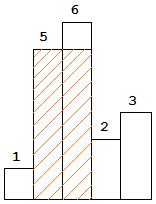
\includegraphics[scale=2.00]{histogram_area}}
\caption{Largest rectangle in histogram}
\label{fig:histogram_area}
\end{figure}

Keep a stack storing the bars in non-decreasing, then calculate the area by popping out the stack to get the currently lowest bar which determines the height of the rectangle.
\\
Core clues:
\begin{enumerate}
\item Maintain the non-decreasing stack. slow performance 
\item Popping triggers the calculation of area
\item Calculate the rectangle width by index diff
\item Post-processing in the end
\end{enumerate}
\newpage
Code:
\begin{python}
def largestRectangleArea(self, height):
    n = len(height)
    gmax = -sys.maxint-1
    stk = []  # store the idx, non-decreasing stack

    for i in xrange(n):
        while stk and height[stk[-1]] > height[i]:
            last = stk.pop()
            if stk:  # calculate area when popping
                area = height[last]*(i-(stk[-1]+1))
            else:
                area = height[last]*i
            gmax = max(gmax, area)

        stk.append(i)

    # after array scan, process the dangling stack
    i = n
    ...

    return gmax
\end{python}


\subsection{All nearest smaller values}\label{allNearestSmaller}
\textbf{Nearest smaller}. Left neighbor of a value $v$ to be the value that occurs prior to $v$, is smaller than $v$, and is closer in position to $v$ than any other smaller value.

For each position in a sequence of numbers, search among the \textit{previous} positions for the last position that contains a smaller value. 

Core clues:
\begin{enumerate}
\item Maintain a \textit{strictly increasing} stack.  
\item If all nearest \textit{larger} values, maintain a \textit{strictly decreasing} stack.  
\end{enumerate}

\begin{python}
def allNearestSmaller(self, A):
    P = [-1 for _ in A]
    stk = []
    for i, v in enumerate(A):
        while stk and A[stk[-1]] >= v: stk.pop()

        if stk:
            P[i] = stk[-1]
        else:
            P[i] = -1  # no preceding smaller value
            
        stk.append(i)  # store the idx or val

    return P
\end{python}

\section{Map}
\subsection{Math relations}
\textbf{1-1 Map}. Mathematically, full projection. One map, dual entries.
\begin{python}
class OneToOneMap(object):
    def __init__(self):
        self.m = {}  # keep a single map

    def set(self, a, b):
        self.m[a] = b
        self.m[b] = a

    def get(self, a):
        return self.m.get(a)
\end{python}
\subsection{Operations}
\runinhead{Sorting by value.} Sort the map entries by values \pyinline{itemgetter}.
\begin{python}
from operators import itemgetter 
sorted(hm.items(), key=itemgetter(1), reverse=True)
\end{python}
